\DocumentMetadata
  {
    lang=en-US,
    pdfversion=2.0,
    pdfstandard=ua-2,
    tagging=on,
  }
\documentclass{article}
\usepackage{incgraph}
\usepackage{tikz}

\begin{document}

\begin{inctext}
Some text
\end{inctext}

Before text

\begin{inctext}
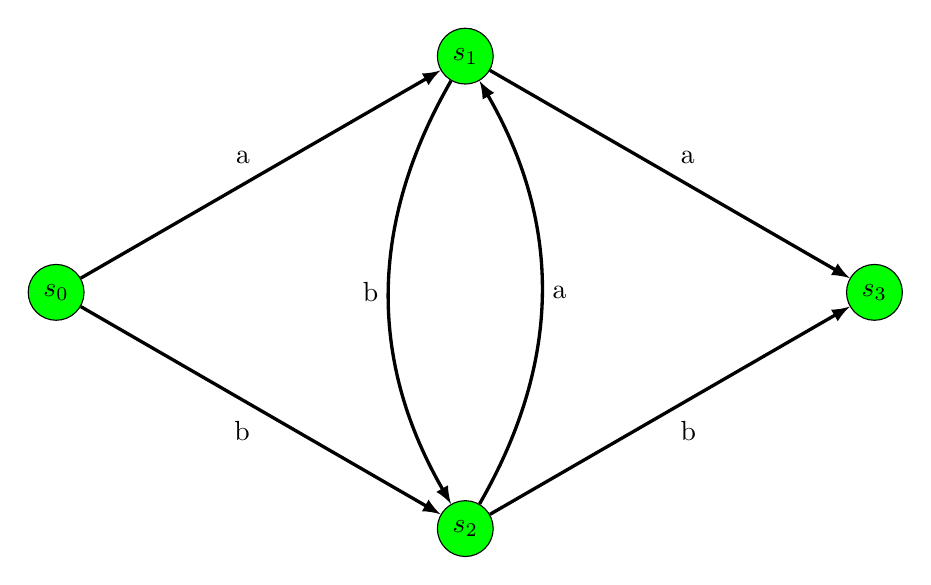
\begin{tikzpicture}[zustand/.style={circle,fill=green,draw},scale=2]
\draw node[zustand] (s0) {$s_0$}
+(30:3cm) node[zustand] (s1) {$s_1$}
++(-30:3cm) node[zustand] (s2) {$s_2$}
+(30:3cm) node[zustand] (s3) {$s_3$};
\path[very thick,-latex]
(s0) edge node[above left] {a} (s1)
edge node[below left] {b} (s2)
(s1) edge[out=-120,in=120] node[left] {b} (s2)
edge node[above right] {a} (s3)
(s2) edge[out=60,in=-60] node[right] {a} (s1)
edge node[below right] {b} (s3);
\end{tikzpicture}
\end{inctext}

After text

\end{document}